% CVPR 2022 Paper Template
% based on the CVPR template provided by Ming-Ming Cheng (https://github.com/MCG-NKU/CVPR_Template)
% modified and extended by Stefan Roth (stefan.roth@NOSPAMtu-darmstadt.de)

\documentclass[10pt,twocolumn,letterpaper]{article}

%%%%%%%%% PAPER TYPE  - PLEASE UPDATE FOR FINAL VERSION
\usepackage[review]{cvpr}      % To produce the REVIEW version
%\usepackage{cvpr}              % To produce the CAMERA-READY version
%\usepackage[pagenumbers]{cvpr} % To force page numbers, e.g. for an arXiv version

% Include other packages here, before hyperref.
\usepackage{graphicx}
\usepackage{amsmath}
\usepackage{amssymb}
\usepackage{booktabs}
\usepackage{array}
\usepackage{url} 
\usepackage[OT1]{fontenc} 
\usepackage{fontspec}
% It is strongly recommended to use hyperref, especially for the review version.
% hyperref with option pagebackref eases the reviewers' job.
% Please disable hyperref *only* if you encounter grave issues, e.g. with the
% file validation for the camera-ready version.
%
% If you comment hyperref and then uncomment it, you should delete
% ReviewTempalte.aux before re-running LaTeX.
% (Or just hit 'q' on the first LaTeX run, let it finish, and you
%  should be clear).
\usepackage[pagebackref,breaklinks,colorlinks]{hyperref}
\usepackage[bottom]{footmisc}


% Support for easy cross-referencing
\usepackage[capitalize]{cleveref}
\crefname{section}{Sec.}{Secs.}
\Crefname{section}{Section}{Sections}
\Crefname{table}{Table}{Tables}
\crefname{table}{Tab.}{Tabs.}


\def\groupID{Group-Q}
\def\subjectNum{COMP6721}
\def\subName{Applied AI } 



\begin{document}
\definecolor{barblue}{RGB}{206,34,34}
\definecolor{groupblue}{RGB}{120,34,34}
\definecolor{linkred}{RGB}{165,0,33}
% \renewcommand\sfdefault{phv}
% \renewcommand\mddefault{mc}
% \renewcommand\bfdefault{bc}
%%%%%%%%% PAPER ID  - PLEASE UPDATE
\def\cvprPaperID{Group-Q} % *** Enter the CVPR Paper ID here
\def\confName{COMP6721}
\def\confYear{2022}

%%%%%%%%% TITLE - PLEASE UPDATE
\title{Lung Disease Clasification - \subName Progress Report}
\author{Rohan Chopra\\
\small 40233019\\
\and
Harman Singh Jolly\\
\small 40204947\\
\and
Harman Preet Kaur\\
\small 40198317\\
\and
Abhishek Handa\\
\small 40231719\\
}
\maketitle
%%%%%%%%% BODY TEXT
\section{Introduction and Problem Statement}
\label{sec:intro}

Early diagnosis of respiratory diseases like pneumonia and COVID-19 leads to decreased mortality rate \cite{daniel2016time} and is a powerful way to manage a pandemic\cite{xu2020facile}. These diseases can be diagnosed using a variety of tests like pulse oximetry, chest x-ray, CT scan\cite{mattsmith2022},  PCR\cite{akhtar1996pcr} however chest X-rays are by far the most accessible\cite{frija2021improve}. Furthermore, the scan is available in minutes making it one of the fastest ways of diagnosis\cite{healthwise2021}. However, the bottleneck with this method is the need for an expert radiologists to evaluate the scan\cite{mehrotra2009radiologists}. Many researchers have tried to solve this problem using deep learning \cite{wang2021deep} but haven't been able to come up with models that can replace radiologists. Small \cite{guefrechi2021deep} and highly imbalanced data \cite{wang2021deep}, along with varying specifications of X-ray scanners are the biggest problems \cite{melissarohman2018} that researchers have faced. Another issue with using deep neural networks in medical settings is its black-box nature\cite{paulblazek2022}, doctors and patients will not trust a model that cannot explain its results\cite{aleksandra2019}. 

This project is an attempt to compare three backbone architectures and lung disease datasets to identify the type of architecture that works best for lung disease classification. The small dataset problem and the issue of different radiographic contrast \cite{andrew2022rad} is mitigated using data augmentation. Imbalanced data will be handled with a combination of using class weights, and a good backbone model. A detailed comparison of results across architectures and datasets along with an explanation of model results will be provided. The final system will use the best model in terms of both efficiency and F1 score allowing rapid diagnosis of lung diseases leading to immediate initiation of treatment, reducing mortality rate.
%-------------------------------------------------------------------------
\section{Proposed Methodologies}
\label{sec:prop_method}
In this study, 12 models, four for each of the three datasets will be trained. The first three models will be trained from scratch and the fourth model will be trained using transfer learning. The hyperparameters will be fixed across models to produce comparable results. Next, hyperparameters will be tuned to find the best model. Finally, the models will be visualized using t-SNE and Grad-CAM \cite{jacobgilpytorchcam} to explain model results. 
\begin{figure}[t]
  \centering
  \includegraphics[width=0.7\linewidth]{pre_proc_img.eps}  
   \caption{Effect of pre-processing on Chest X-ray images.}
   \vspace{-1em}
   \label{fig:pre_proc_img}
\end{figure}
Before training, the images were pre-processed using histogram equalization and Gaussian blur with a 5x5 filter as Giełczyk \etal \cite{gielczyk2022pre} showed that this improved the F1 score by 4\% for chest X-ray classification. Visually, the contrast of the scan improved and allowed irregularities to stand out as shown in \cref{fig:pre_proc_img}. Next, the scans were divided into train, validation and test with the 70:15:15 split. During training, images were augmented using RandomHorizontalFlip, RandomAdjustSharpness, and RandomAutocontrast in Pytorch \cite{transforms} to increase the number of images the model gets to learn from. To train the model, cosine annealing with warm restarts \cite{loshchilov2016sgdr} was used along with the Adam optimizer \cite{kingma2014adam} and the cross entropy loss function. 
\begin{figure}[t]
  \centering
  \includegraphics[width=1\linewidth]{samp_img.eps}  
   \caption{Sample images of Chest X-rays.}
   \vspace{-0.5em}
   \label{fig:sample_img}
\end{figure}

\begin{table}
  \centering
  \begin{tabular}{p{2.9cm}|p{2.3cm}|wc{0.8cm}|p{0.8cm}}
    \toprule
    Dataset & No. of Images & Classes & Size\\
    \midrule
    COVID\cite{RAHMAN2021104319,9144185,kagglecovid} & 10k:3.6k:1.3k & 3 & 299\textsuperscript{2}\\
    \midrule
    Pneumonia\cite{kermany2018labeled,kagglepneu} & 3k:1.5k:1.5k & 3 & 224\textsuperscript{2}\\
    \midrule
    Chest X-Ray8\cite{wang2017chestx,kaggle8} & 25k:12k:6k:5k :3k:2.7k:2.6k & 7 & 1024\textsuperscript{2}\\
    \bottomrule
  \end{tabular}
  \caption{Shortlisted Datasets.}
  \vspace{-1.5em}
  \label{tab:selDataset}
\end{table}
\textbf{Datasets:} (\cref{tab:selDataset}) with varying disease types were chosen to ensure model robustness. Other criteria included the \textit{number of images per class} and \textit{image quality} as noisy scans can lead to mis-diagnosis\cite{sivakumar2012computed}. 
The \textbf{COVID} dataset was created using 43 \cite{covidpneumonia2020data} different publications. \cite{RAHMAN2021104319,9144185,kagglecovid} X-rays with widespread, hazy, and irregular ground glass opacities are of the COVID-19 class \cite{jacobi2020portable}. Whereas, the ones with haziness only in the lower regions \cite{zhan2021clinical} are viral pneumonia cases as shown in \cref{fig:sample_img}.
The \textbf{Pneumonia}, dataset contains scans from pediatric patients. \cite{kermany2018labeled,kagglepneu} Scans with one white condensed area affecting only one side of the lungs are tagged bacterial pneumonia\cite{areviral}. X-rays which show bilateral patchy areas of consolidation are classified as viral pneumonia\cite{guo2012radiological}. 
\textbf{Chest X-ray 8} dataset was released by NIH \cite{chestxray2017data} with over 100k chest X-ray images and their radiological reports which Wang \etal \cite{wang2017chestx} used to create disease labels through NLP. \cite{kaggle8} It contains 15 classes but only 7 were chosen for this study. Furthermore, normal class images were undersampled to choose only one scan per patient. 

\textbf{Backbone Architectures:} (\cref{tab:selArch}) of various configuration and blocks were chosen. Other selection criteria were the \textit{number of trainable parameters}, important as total training time and hardware resources are limited for this project and the \textit{top 5 classification accuracy} on the ImageNet 1K benchmark dataset.
\begin{table}
  \centering
  \begin{tabular}{p{1.7cm}|p{1cm}|p{1cm}|p{1cm}|p{1cm}}
  \toprule
  Arch. & Params (Mil.) & Layers & FLOPS (Bil.) & Imagenet Acc.\\
  \midrule
  MobileNet & 5.5 & 18 & 8.7 & 92.6\\
  \midrule
  EfficientNet & 7.8 & 25 & 25.8 & 94.9\\
  \midrule
  Resnet & 21.8 & 34 & 153.9 & 91.4\\
  \bottomrule
  \end{tabular}
  \caption{Shortlisted Backbone Architectures.}
  \vspace{-1.5em}
  \label{tab:selArch}
\end{table}
\textbf{ResNet 34}: residual learning network with 34 layers that are made possible by skip connections. The 34 layer variant was chosen to decrease training time. \cite{he2016deep}
\textbf{MobileNet V3 Large}: uses depthwise separable convolution from MobileNet V2 \cite{sandler2018mobilenetv2} along with squeeze-excitation blocks in residual layers from MnasNet \cite{tan2019mnasnet}. Howard \etal \cite{howard2019searching} also used network architecture search to find the most effective model. The large configuration was chosen to not compromise on the prediction accuracy.
\textbf{EfficientNet B1}: uses compound scaling to scale the model by depth, width and resolution. The B1 version was chosen to have faster training without compromising on the accuracy. \cite{tan2019efficientnet}
\section{Attempts at Solving the Problem} 
\label{sec:method}
Two datasets in this study had a very small number of samples which caused the models to overfit early. To mitigate this, random contrast and sharpness adjustment \cite{nanni2021comparison} data augmentation techniques were used. Some scans in the datasets were anterior-posterior while some others were posterior-anterior and using the horizontal flip data augmentation would make the model invariant to these differences\cite{botev2022regularising}.
Inception was the first model trained and each epoch took over 1 hour. To reduce the training time, the X-ray images were resized, pre-processed and split into train, test and validation sets separately. Furthermore, EfficientNet, MobileNet and ResNet 34 were chosen as they have a considerably low number of learnable parameters. Now each epoch is taking less than 4 minutes. 

Nine models were trained from scratch and the training, validation F1 score and loss can be seen in \cref{fig:acc_loss_sep}. From the plots it is clear that going from a smaller architecture to a bigger architecture, makes the model start to overfit earlier. Another interesting observation is that cosine annealing impacted the loss of MobileNet the most every 10 epochs due to warm restarts. From the graphs it can be seen that all three datasets had similar performance across models when trained for a high number of epochs. The X-ray 8 dataset performed the worst among the three datasets which could be due to the high number of classes as compared to the other datasets. Surprisingly, the pneumonia dataset performed worse than the COVID + pneumonia dataset which indicates that COVID cases are easier to distinguish from pneumonia cases. 

\begin{figure}[t]
  \centering
  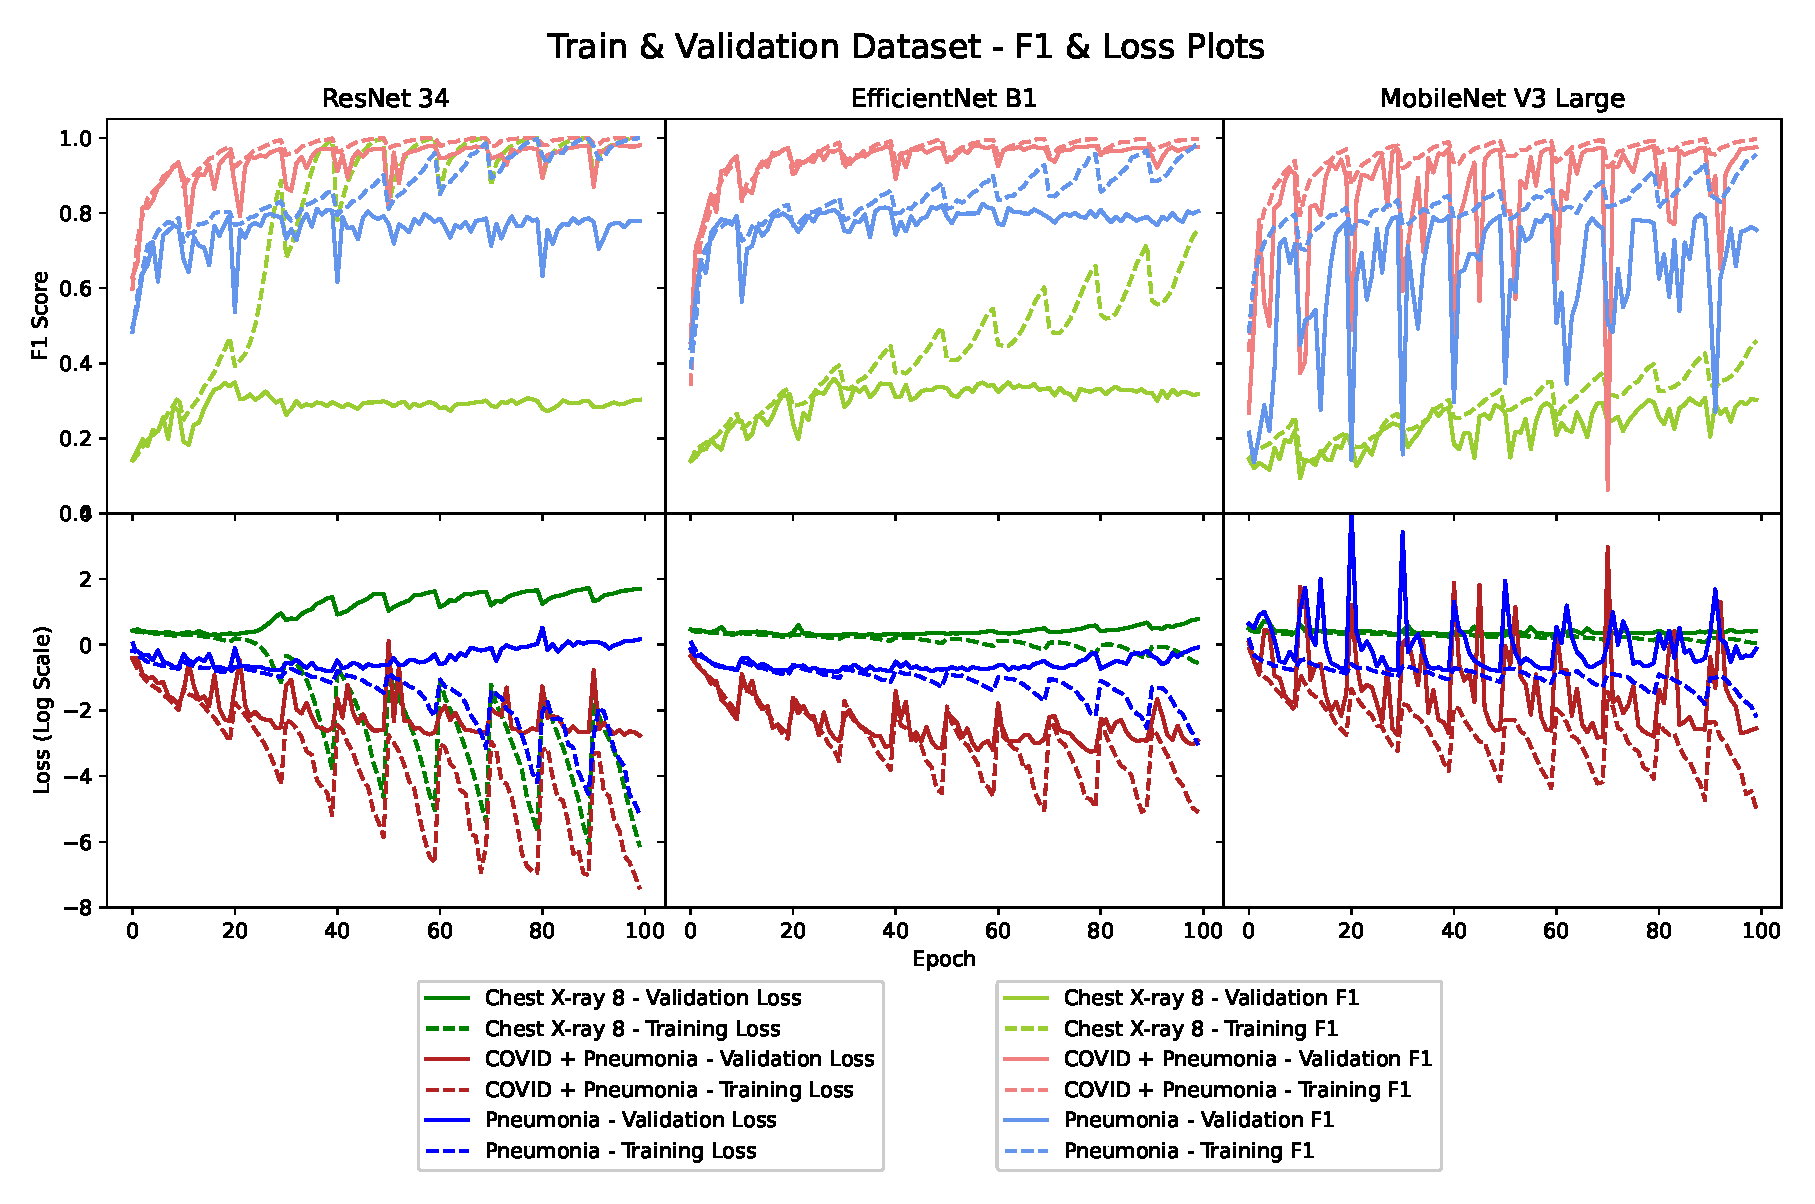
\includegraphics[width=1\linewidth]{f1_loss_separate.eps}  
   \caption{Train \& Val F1 \& Loss plots for the 9 models.}
   \vspace{-1em}
   \label{fig:acc_loss_sep}
\end{figure}

%-------------------------------------------------------------------------
\section{Future Improvement}
\label{sec:future}
The model with best validation loss is being saved to evaluate the test set but, going forward, the models will be trained for 50 epochs to save time as all the models start to overfit after that point. Class weights will be explored to improve model performance and a confusion matrix of the test set will be produced to understand model mis-classifications. One model for each dataset will be trained using transfer learning and its performance will be compared with models trained from scratch. Ablation study will be performed to see how different hyperparameters affect the F1 score of the models. Finally, t-SNE \cite{van2008visualizing} and grad-CAM \cite{jacobgilpytorchcam} will be used to visualize the trained models.

%%%%%%%%% REFERENCES
\clearpage
{\small
\bibliographystyle{ieee_fullname}
\bibliography{egbib}
}
\end{document}